\documentclass{standalone}
\usepackage{tikz,pgfplots}
\pgfplotsset{compat=newest}
\begin{document}

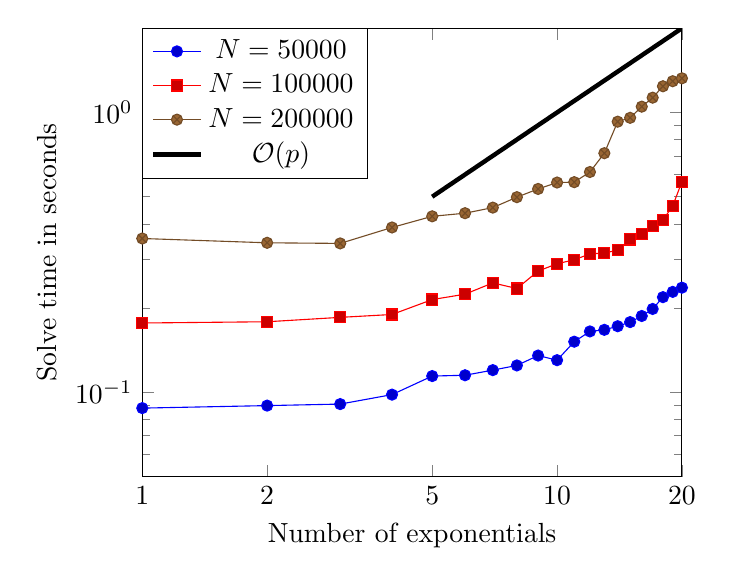
\begin{tikzpicture}
\begin{loglogaxis}[
	xlabel={Number of exponentials},
	ylabel={Solve time in seconds},
	xmin=1, xmax=20,
	ymin=5e-2, ymax=2,
%	log x ticks with fixed point,
	xticklabel style={/pgf/number format/.cd,fixed,precision=2},
    xticklabel={%
      \pgfmathfloatparsenumber{\tick}%
      \pgfmathfloatexp{\pgfmathresult}%
      \pgfmathprintnumber{\pgfmathresult}%
	  },
	  xtick={1, 2, 5,  10, 20},
	  legend style={
    		at={(0.0,1.0)},
			anchor=north west},
%	xticklabel=\pgfmathparse{10^\tick}\pgfmathprintnumber{\pgfmathresult}
]
%Fast N=50000
\addplot
coordinates{
(1, 0.087815) (2, 0.089646) (3, 0.090774) (4, 0.098116) (5, 0.114305) (6, 0.115081) (7, 0.120031) (8, 0.124745) (9, 0.135322) (10, 0.130269) (11, 0.151676) (12, 0.165051) (13, 0.16722) (14, 0.172262) (15, 0.178218) (16, 0.187403) (17, 0.198575) (18, 0.218821) (19, 0.228515) (20, 0.236572) 
};
\addlegendentry{$N=50000$}
%Fast N=100000
\addplot
coordinates{
(1, 0.17689) (2, 0.17872) (3, 0.185307) (4, 0.189716) (5, 0.214471) (6, 0.22423) (7, 0.246022) (8, 0.234882) (9, 0.271075) (10, 0.288088) (11, 0.297481) (12, 0.312287) (13, 0.314563) (14, 0.322186) (15, 0.351757) (16, 0.368492) (17, 0.391859) (18, 0.412696) (19, 0.463227) (20, 0.565839) 
};
\addlegendentry{$N=100000$}
%Fast N=200000
\addplot
coordinates{
(1, 0.354527) (2, 0.342209) (3, 0.340521) (4, 0.388258) (5, 0.425494) (6, 0.43657) (7, 0.457093) (8, 0.498104) (9, 0.532948) (10, 0.56189) (11, 0.563565) (12, 0.612678) (13, 0.715281) (14, 0.92696) (15, 0.95683) (16, 1.04894) (17, 1.129441) (18, 1.24063) (19, 1.29322) (20, 1.3245) 
};
\addlegendentry{$N=200000$}
%O(p) scaling
\addplot[ultra thick, no marks]
coordinates{
(5, 0.5) (20, 2)
};
\addlegendentry{$\mathcal{O}(p)$}
\end{loglogaxis}
\end{tikzpicture}
\end{document}